% !TeX root = ../main.tex

\chapter{Methodik}
\label{chapter:method}

\section{Methodischer Rahmen}
Diese Forschungsarbeit verfolgt einen gestaltungsorientierten Ansatz im Sinne von Design Science Research (DSR), welcher sich insbesondere für Forschungsvorhaben eignet, bei denen nicht ausschließlich bestehende Phänomene beschrieben oder erklärt werden sollen (Behavioral Science Research), sondern Lösungen für praxisnahe Problemstellungen entwickelt und wissenschaftlich evaluiert werden. Das Forschungsdesign orientiert sich dabei am DSR-Framework nach Hevner et al. \cite{hevner2004design} und nutzt das Prozessmodell nach Peffers et al. \cite{peffers2007design} zur Strukturierung des konkreten Forschungsvorgehens.

\subsection{DSR-Framework}
\label{subsec:DSR_Framework}

Abbildung \ref{fig:Hevner} zeigt das DSR-Framework nach Hevner et al. \cite{hevner2004design}:

\begin{figure}[ht]
    \centering
    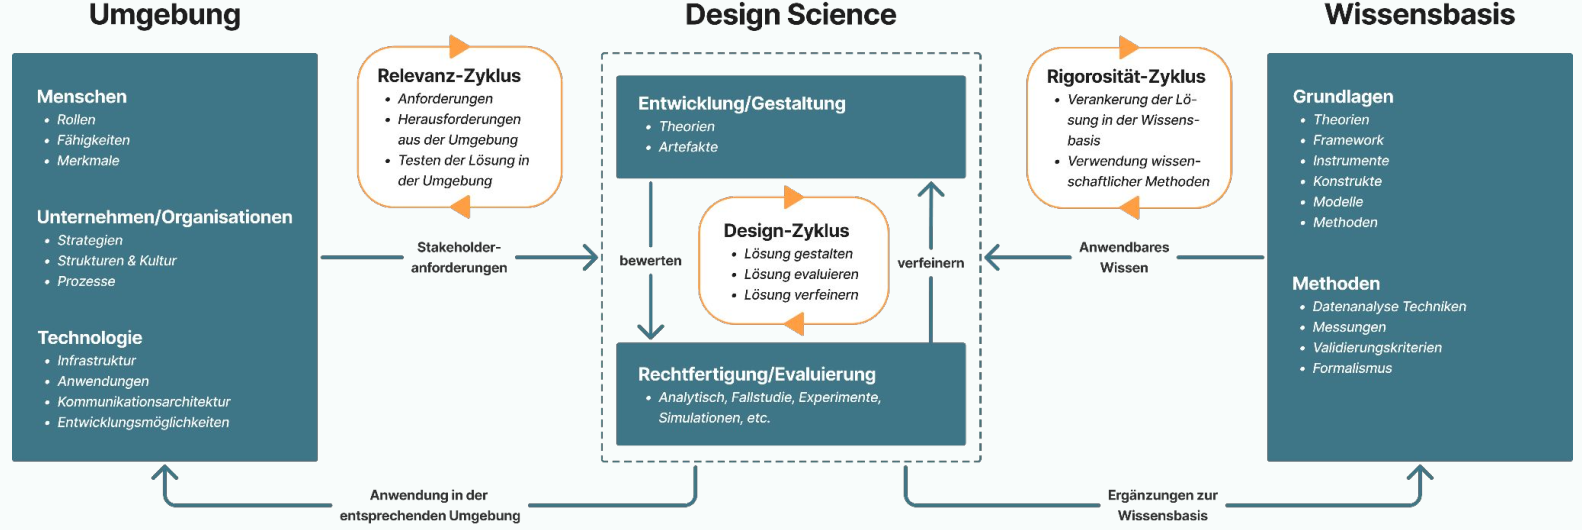
\includegraphics[width=1\textwidth]{images/method/Framework_DSR.png}
    \caption{DSR-Framework/Cycles nach Hevner et al.}
    \label{fig:Hevner}
    \medskip
    {\footnotesize Quelle: Entnommen aus \cite[S.~6]{dogangun2025dsr}.}
\end{figure}

Die einzelnen Bestandteile des Frameworks werden im Folgenden nicht abstrakt,
sondern anhand ihrer Entsprechungen innerhalb dieser Forschungsarbeit
beschrieben. 

Die Wissensbasis auf der rechten Seite des Frameworks wird insbesondere durch die in Kapitel \ref{chapter:theory} aufgearbeiteten
theoretischen Grundlagen und den bestehenden Forschungsstand repräsentiert. Dazu zählen sowohl Erkenntnisse zur sicherheitskritischen
Mensch-Maschine-Interaktion und zu relevanten Human Factors als auch bestehende Forschungsarbeiten zur Informationsvermittlung, zum Training und zum Onboarding von Fahrassistenzsystemen. Über den Rigorositäts-Zyklus fließen diese bestehenden Erkenntnisse in die Entwicklung der Gestaltungslösung ein. Gleichzeitig sollen die im Rahmen der Entwicklung und Evaluation gewonnenen Erkenntnisse einen Beitrag zur bestehenden Wissensbasis leisten.

Die Umgebung auf der linken Seite des Frameworks umfasst den praktischen
Anwendungskontext des zu untersuchenden Problems. Für die vorliegende Arbeit
wird dieser insbesondere durch Fahrer*innen, Fahrassistenzsysteme, bestehende
Informationsdefizite sowie den sicherheitskritischen Fahrzeugkontext
repräsentiert. Der Relevanz-Zyklus stellt die Verbindung zwischen diesem
Anwendungskontext und dem Forschungsprozess her. Dies erfolgt zunächst durch
die Untersuchung bestehender Probleme und der Bedarfe potenzieller
Nutzer*innen und später durch die Evaluation der entwickelten Lösung in einem
kontrollierten, fahrnahen Anwendungskontext.

Im Zentrum des Frameworks steht der Design-Zyklus, der die Entwicklung und Evaluation eines Artefakts miteinander verknüpft. In der vorliegenden Arbeit umfasst dieser die Ableitung von Gestaltungsanforderungen, die partizipative Entwicklung eines In-Car-Onboarding-Konzepts, dessen prototypische Umsetzung sowie die anschließende Evaluation im Fahrsimulator. Aufgrund des zeitlichen und inhaltlichen Umfangs der Masterarbeit wird dabei kein mehrfacher vollständiger Entwicklungs- und Evaluationszyklus durchlaufen. Die aus der Evaluation resultierenden Erkenntnisse dienen daher nicht einer weiteren Überarbeitung und erneuten Evaluation innerhalb dieser Arbeit, sondern werden als Ausgangspunkt für mögliche zukünftige Iterationen diskutiert.

Das DSR-Framework von Hevner et al. \cite{hevner2004design} ermöglicht eine übergeordnete Einordnung der Forschungsarbeit in Anwendungskontext und wissenschaftliche Wissensbasis, strukturiert die einzelnen Forschungsaktivitäten jedoch nicht wie ein Prozessmodell. Aus diesem Grund soll im folgenden Abschnitt das DSR-Prozessmodell nach Peffers \cite{peffers2007design} zur Beantwortung dieser noch offenen Fragestellung verwendet werden.

\subsection{DSR-Prozessmodell}
\label{subsec:DSR_Prozessmodell}

Abbildung \ref{fig:Peffers} zeigt das DSR-Prozessmodell nach Peffers et al. \cite{peffers2007design}.

\begin{figure}[ht]
    \centering
    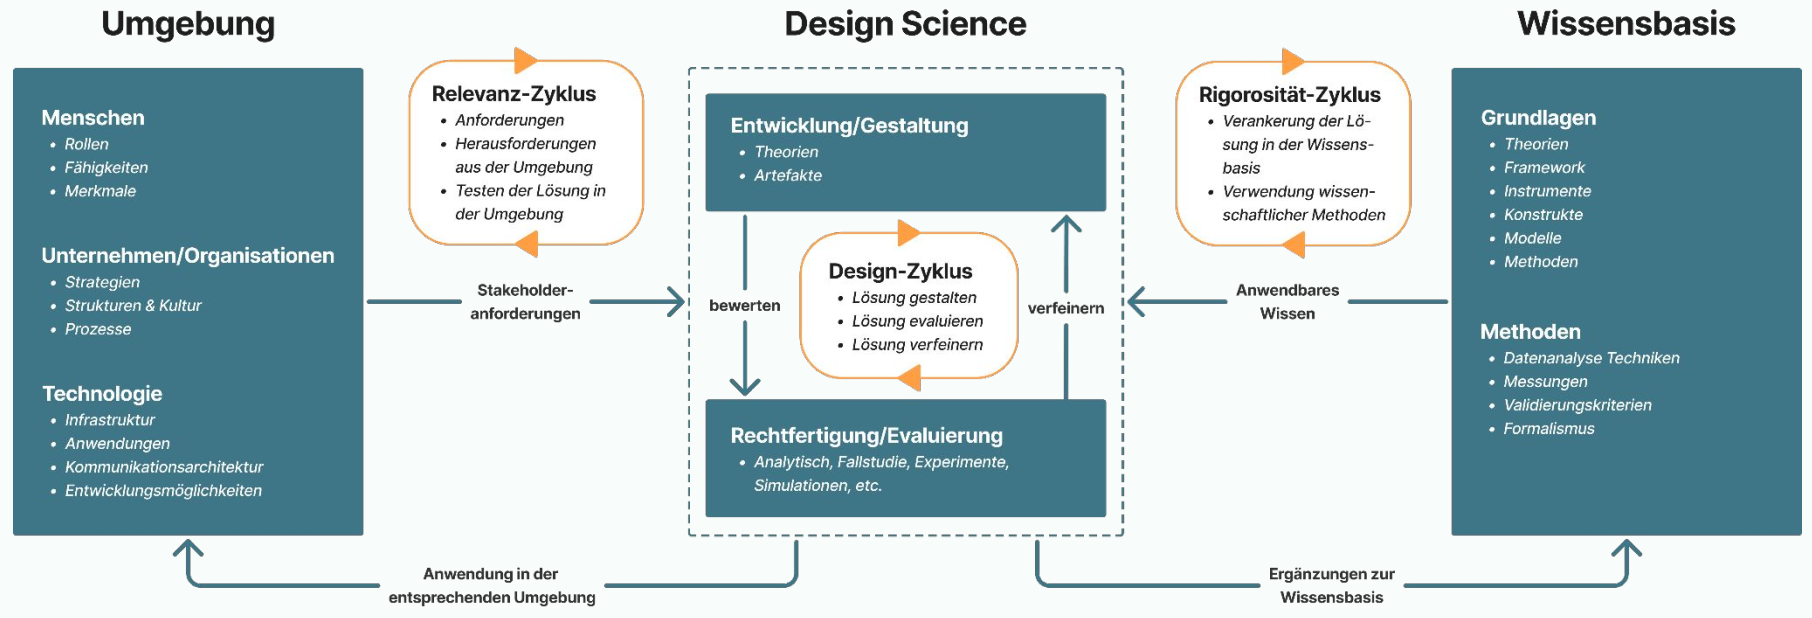
\includegraphics[width=1\textwidth]{images/method/Modell_DSR.png}
    \caption{Zyklischer DSR-Prozess nach Peffers et al.}
    \label{fig:Peffers}
    \medskip
    {\footnotesize Quelle: Entnommen aus \cite[S.~53]{dogangun2025dsr}.}
\end{figure}

Das Modell konkretisiert DSR in sechs aufeinander bezogenen Aktivitäten, wobei der Ablauf nicht als strikt linear zu verstehen ist. Die einzelnen Aktivitäten werden in der vorliegenden Arbeit direkt auf den Untersuchungsgegenstand übertragen und dienen der Strukturierung des konkreten Forschungsvorgehens.

Die Aktivität 'Problemidentifikation und Motivation' umfasst die Untersuchung des bestehenden Forschungsstands sowie die Erhebung der Erfahrungen, Erwartungen und Informationsbedarfe potenzieller Nutzer*innen. Ziel ist es, die zugrunde liegende Problemstellung sowohl aus wissenschaftlicher als auch aus Nutzer*innenperspektive zu konkretisieren und ihre Relevanz für die Entwicklung eines In-Car-Onboardings zu begründen. Darauf aufbauend werden im Rahmen der Aktivität 'Zielsetzung der Lösung' die Erkenntnisse aus Literatur und Nutzer*inneninterviews systematisch zusammengeführt und in konkrete Gestaltungsanforderungen für das In-Car-Onboarding überführt. Diese Anforderungen dienen als Grundlage für die nachfolgende Gestaltung des Artefakts. Die Aktivität 'Design und Entwicklung' umfasst die partizipative Entwicklung eines In-Car-Onboarding-Konzepts sowie dessen prototypische Umsetzung. Die zuvor abgeleiteten Gestaltungsanforderungen werden hierbei in eine konkrete Gestaltungslösung überführt. Im Rahmen der 'Demonstration' wird der entwickelte Prototyp in definierten Fahrsituationen innerhalb eines Fahrsimulators eingesetzt. Dadurch wird die Anwendung des Artefakts in einem kontrollierten, fahrnahen Nutzungskontext ermöglicht. Die anschließende 'Evaluation' untersucht, inwiefern der entwickelte Prototyp die zuvor definierten Zielsetzungen erfüllt. Dabei wird insbesondere betrachtet, in welchem Umfang das In-Car-Onboarding das Systemverständnis sowie ein angemessenes Nutzungsverhalten unterstützt. Die Aktivität 'Kommunikation' erfolgt übergreifend durch die wissenschaftliche Dokumentation, Darstellung und Diskussion des Forschungsvorgehens und der gewonnenen Ergebnisse im Rahmen dieser Masterarbeit. Tabelle \ref{tab:dsr-aktivitaeten} zeigt die Übertragung der DSR-Aktivitäten auf die vorliegende Forschungsarbeit noch einmal übersichtlich.

{
\footnotesize
\renewcommand{\arraystretch}{1.2}
\setlength{\tabcolsep}{3pt}

\begin{xltabular}{\textwidth}{
    |P{0.30\textwidth}
    |Y|
}

\hline

\textbf{DSR-Aktivität} &
\textbf{Umsetzung in dieser Forschungsarbeit}
\\
\hline
\endfirsthead

\multicolumn{2}{c}{%
    \tablename\ \thetable{} -- Fortsetzung%
}
\\
\hline

\textbf{DSR-Aktivität} &
\textbf{Umsetzung in dieser Forschungsarbeit}
\\
\hline
\endhead

\hline
\multicolumn{2}{r}{Fortsetzung auf der nächsten Seite}
\\
\endfoot

\endlastfoot


Problemidentifikation und Motivation &
Analyse des bestehenden Forschungsstands sowie qualitative Nutzer*inneninterviews zur Erfassung von Problemen, Erfahrungen, Erwartungen und Informationsbedarfen
\\
\hline

Zielsetzung der Lösung &
Systematische Zusammenführung der Erkenntnisse aus Literatur und Interviews sowie Ableitung konkreter Gestaltungsanforderungen für das In-Car-Onboarding
\\
\hline

Design und Entwicklung &
Partizipative Entwicklung eines In-Car-Onboarding-Konzepts und prototypische Umsetzung auf Basis der zuvor abgeleiteten Gestaltungsanforderungen
\\
\hline

Demonstration &
Einsatz des entwickelten Prototyps in definierten Fahrsituationen innerhalb des Fahrsimulators
\\
\hline

Evaluation &
Bewertung des Prototyps hinsichtlich der zuvor definierten Zielsetzungen, insbesondere in Bezug auf Systemverständnis und angemessenes Nutzungsverhalten
\\
\hline

Kommunikation &
Wissenschaftliche Dokumentation, Darstellung und Diskussion des Forschungsvorgehens und der gewonnenen Ergebnisse im Rahmen der Masterarbeit
\\
\hline

\caption{Übertragung der DSR-Aktivitäten nach Peffers et al. auf die vorliegende Forschungsarbeit}
\label{tab:dsr_aktivitaeten}
\\

\end{xltabular}
}

Die nachfolgenden Abschnitte beschreiben die methodische Ausgestaltung der DSR-Aktivitäten im Detail.

\section{Problemidentifizierung und Motivation}
\label{sec:Methodik_Phase_eins}

\subsection{Literaturrecherche}
\label{subsec:Literaturrecherche}

Die in Kapitel \ref{chapter:theory} vorgestellte wissenschaftliche Aufarbeitung des Problemraums erfolgte im Rahmen einer strukturierten Literaturrecherche, deren Auswahlprozess sich an den Grundprinzipien des PRISMA-Ansatzes \cite{page2021prisma} orientierte. 

\subsubsection{Identifikation}
\label{subsubsec:Identifikation}

Die Recherche wurde in den Datenbanken 'IEEE Xplore', 'ACM Digital Library' sowie 'Google Scholar' durchgeführt. Für die Suche wurden mehrere thematische Blöcke gebildet und Suchbegriffe abgeleitet. Typischerweise wurde mindestens ein Begriff aus dem Block System/Funktion mit Begriffen aus den Bereichen Onboarding/Lernen, Interface/Gestaltung oder Zielgrößen kombiniert. Die konkrete Syntax wurde an die technischen Möglichkeiten der jeweiligen Datenbank angepasst. Ergänzend zur datenbankgestützten Recherche wurde eine Vorwärts- und Rückwärtssuche durchgeführt. Hierbei wurden die Literaturverzeichnisse besonders relevanter Publikationen auf weitere einschlägige Quellen geprüft und Publikationen berücksichtigt, die zentrale Arbeiten des Themenfelds zitieren. Tabelle \ref{tab:literatur_suchbegriffe} zeigt eine Übersicht der verwendeten Suchbegriffe.

{
\footnotesize
\renewcommand{\arraystretch}{1.2}
\setlength{\tabcolsep}{3pt}

\begin{xltabular}{\textwidth}{
    |P{0.20\textwidth}
    |P{0.24\textwidth}
    |Y|
}

\hline

\textbf{Block} &
\textbf{Inhaltlicher Fokus} &
\textbf{Verwendete Suchbegriffe}
\\
\hline
\endfirsthead

\multicolumn{3}{c}{%
    \tablename\ \thetable{} -- Fortsetzung%
}
\\
\hline

\textbf{Block} &
\textbf{Inhaltlicher Fokus} &
\textbf{Verwendete Suchbegriffe}
\\
\hline
\endhead

\hline
\multicolumn{3}{r}{Fortsetzung auf der nächsten Seite}
\\
\endfoot

\endlastfoot


A: System/Funktion &
Fahrassistenz und Automatisierung &
ADAS, advanced driver assistance system*, driver assistance system*,
driver assistance, adaptive cruise control, ACC,
lane keeping assist, lane centering, parking assist
\\
\hline

B: Onboarding/Lernen &
Einführung in die Nutzung und Wissensvermittlung &
onboarding, user onboarding, training, driver training,
tutorial*, instruction*, education, familiarization,
information provision, user manual, owner's manual
\\
\hline

C: Interface/Gestaltung &
Gestaltung und Vermittlungsform &
in-car HMI, in-vehicle HMI, automotive HMI,
human-machine interface, human-vehicle interaction,
interaction design, UX, multimodal interface,
AR tutorial, explanation, feedback
\\
\hline

D: Zielgrößen &
Sichere, korrekte und angemessene Nutzung &
safe use, correct use, appropriate use, misuse,
disuse, overreliance, overtrust, trust calibration,
mental model*, situation awareness, system understanding,
comprehension, understanding, task performance,
user acceptance
\\
\hline

E: Nutzer*innen/Kontext &
Zielgruppe und Nutzungssituation &
first-time users, novice users, drivers, everyday use,
real-world use, take-over, monitoring, driver engagement
\\
\hline

\caption{Thematische Suchblöcke und verwendete Suchbegriffe der Literaturrecherche}
\label{tab:literatur_suchbegriffe}
\\

\end{xltabular}
}

Darüber hinaus wurden die in Tabelle \ref{tab:literatur_einschlusskriterien} gezeigten Ein- und Ausschlusskriterien definiert, um die Relevanz der Suchergebnisse für den Forschungsgegenstand gewährleisten zu können. 

{
\footnotesize
\renewcommand{\arraystretch}{1.2}
\setlength{\tabcolsep}{3pt}

\begin{xltabular}{\textwidth}{
    |P{0.22\textwidth}
    |P{0.24\textwidth}
    |P{0.22\textwidth}
    |Y|
}

\hline

\textbf{Kriterium} &
\textbf{Beschreibung} &
\textbf{Inkludiert} &
\textbf{Exkludiert}
\\
\hline
\endfirsthead

\multicolumn{4}{c}{%
    \tablename\ \thetable{} -- Fortsetzung%
}
\\
\hline

\textbf{Kriterium} &
\textbf{Beschreibung} &
\textbf{Inkludiert} &
\textbf{Exkludiert}
\\
\hline
\endhead

\hline
\multicolumn{4}{r}{Fortsetzung auf der nächsten Seite}
\\
\endfoot

\endlastfoot


Zeitraum: Kernliteratur &
Aktueller Forschungsstand und empirische Arbeiten &
2020--2026 &
Publikationen vor 2020, sofern keine begründete Ausnahme vorliegt
\\
\hline

Zeitraum: Hintergrundliteratur &
Ergänzende Arbeiten zur Einordnung des Forschungsfelds &
2015--2019 &
Publikationen vor 2015, sofern keine grundlegende Relevanz besteht
\\
\hline

Zeitraum: Ausnahmen &
Grundlagenliteratur, etablierte Modelle, Normen oder zentrale ältere Arbeiten &
Begründete Einzelfälle vor 2015 &
--
\\
\hline

Sprache &
Sprachliche Zugänglichkeit der Publikationen &
Deutsch und Englisch &
Andere Sprachen
\\
\hline

Publikationstyp &
Wissenschaftliche Qualität und Nachvollziehbarkeit &
Peer-reviewte Zeitschriften- und Konferenzbeiträge &
Reports, Policy Papers, Working Papers, Newsletter, Regierungsdokumente, Patente und nichtwissenschaftliche Veröffentlichungen
\\
\hline

Quellentyp &
Berücksichtigung wissenschaftlich geeigneter Publikationsformen &
Zeitschriftenartikel, begutachtete Konferenzbeiträge, Bücher und Buchkapitel &
--
\\
\hline

Volltextzugang &
Ausreichende Grundlage für die inhaltliche Bewertung &
Publikationen mit verfügbarem Volltext &
Kein Volltextzugang trotz angemessener Beschaffungsversuche
\\
\hline

Thematische Relevanz &
Bezug zur Forschungsfrage und zum Untersuchungsgegenstand &
Arbeiten zu Fahrassistenzsystemen, Onboarding, Training, Informationsvermittlung, HMI, Systemverständnis oder angemessener Nutzung &
Arbeiten ohne erkennbaren Bezug zur Forschungsfrage
\\
\hline

\caption{Ein- und Ausschlusskriterien der Literaturrecherche}
\label{tab:literatur_einschlusskriterien}
\\

\end{xltabular}
}

\subsubsection{Vorauswahl}
\label{subsubsec:Vorauswahl}

Die identifizierten Publikationen wurden zunächst anhand von Titel und Abstract auf ihre thematische Relevanz geprüft. Publikationen, die mehrfach über unterschiedliche Datenbanken identifiziert wurden, wurden mithilfe eines Python-basierten Verfahrens zur Dublettenerkennung bereinigt.

\subsubsection{Eignungsprüfung}
\label{subsubsec:Eignungsprüfung}
Bei ausreichender Relevanz erfolgte anschließend eine Prüfung des Volltexts anhand der definierten Ein- und Ausschlusskriterien auf einer tieferen Detailebene. 

\subsubsection{Aufnahme}
\label{subsubsec:Aufnahme}
Die auf diese Weise ausgewählten Publikationen wurden anschließend inhaltlich hinsichtlich ihrer Relevanz für die Problemstellung der vorliegenden Arbeit ausgewertet. Im Fokus standen insbesondere Erkenntnisse zu Nutzungsschwierigkeiten und Fehlanwendungen von Fahrassistenzsystemen,
relevanten Human Factors, bestehenden Informations- und Trainingsansätzen sowie möglichen Gestaltungsansätzen für die Vermittlung von Systemfunktionen und -grenzen. 

\subsection{Qualitative Nutzer*inneninterviews}
\label{subsec:Qualitative_Interviews}

Ergänzend zur Literaturrecherche wurden qualitative Interviews mit der Zielgruppe des Forschungsgegenstands durchgeführt. Ziel war es, Erfahrungen, Unsicherheiten und Schwierigkeiten im Umgang mit Fahrassistenzsystemen sowie bestehende Informations- und Lernbedarfe zu erfassen. Im Fokus standen dabei insbesondere die bisherige Nutzung und Aneignung von Fahrassistenzsystemen, das Verständnis von Funktionen und Systemgrenzen sowie Erwartungen an die Vermittlung relevanter Informationen. Darüber hinaus sollten Präferenzen hinsichtlich des Zeitpunkts und der Form eines möglichen In-Car-Onboardings erhoben werden. Die Interviews ergänzen damit die aus der Literatur gewonnenen Erkenntnisse um die Perspektive potenzieller Nutzer*innen und bilden eine empirische Grundlage für die spätere Ableitung von Gestaltungsanforderungen.

\subsubsection{Stichprobe und Rekrutierung}
\label{subsubsec:Stichprobe_und_Rekrutierung}

Die Zielgruppe der Interviews bildeten Personen mit einer innerhalb der Europäischen Union gültigen Fahrerlaubnis. Außerdem wurde eine Zusammensetzung angestrebt, welche divers anhand der Erfahrungsstände im Umgang mit Fahrzeugen und des biologischen Alters ist, um unterschiedliche Perspektiven beachten zu können. Insgesamt nahmen 11 Personen an den qualitativen Interviews teil, darunter fünf weibliche und sechs männliche Personen. Die Altersspanne umfasste einen Bereich von 25 bis 75 Jahren. Die Rekrutierung erfolgte über das persönliche Umfeld und universitäre Kontaktmöglichkeiten.

\subsubsection{Interviewleitfaden}
\label{subsubsec:Interviewleitfaden}

Die Datenerhebung erfolgte mithilfe eines halbstrukturierten Interviewleitfadens. Diese Interviewform wurde gewählt, um einerseits vergleichbare Themenbereiche bei allen Teilnehmenden abzudecken und andererseits ausreichend Offenheit für individuelle Erfahrungen, Erläuterungen und Nachfragen zu gewährleisten.

Der Leitfaden umfasste zunächst Fragen zur bisherigen Erfahrung mit Fahrassistenzsystemen und zum jeweiligen Nutzungskontext. Anschließend wurden die erste Nutzung entsprechender Systeme, bisherige Formen der Informationsvermittlung und die persönliche Aneignung der Funktionsweise thematisiert. Weitere Fragen bezogen sich auf das Verständnis der Systemfunktion und -grenzen sowie auf Erwartungen und Präferenzen hinsichtlich eines möglichen In-Car-Onboardings.

Die Reihenfolge der Fragen diente dabei als Orientierung und konnte abhängig vom Gesprächsverlauf angepasst werden. Vertiefende Nachfragen wurden eingesetzt, um relevante Aussagen näher zu konkretisieren. Der vollständige Interviewleitfaden ist in Anhang \ref{sec:interviewleitfaden} dokumentiert.

\subsubsection{Durchführung}
\label{subsubsec:Durchführung}

Die Interviews wurden im Zeitraum vom 07.08. bis zum 14.08.2026 durchgeführt und dauerten jeweils ungefähr 30 Minuten. Die Gespräche fanden sowohl in Präsenz als auch Online statt. Vor Beginn des Interviews wurden die Teilnehmenden über Ziel und Ablauf der Untersuchung sowie den Umgang mit den erhobenen Daten informiert.
Alle Interviews wurden mit Einverständnis der Teilnehmenden aufgezeichnet und anschließend für die qualitative Auswertung mithilfe von Whisper \cite{radford2022whisper} transkribiert. Personenbezogene Angaben wurden im Rahmen der Aufbereitung anonymisiert und alle Texte noch einmal manuell überarbeitet. 

\subsubsection{Kodierung und Auswertung}
\label{subsubsec:Kodierung_und_Auswertung}

Im Rahmen der Kodierung und Auswertung wurde eine qualitative Inhaltsanalyse nach Kuckartz \cite{kuckartz2014mixed} praktiziert. Die Arbeiten wurden mithilfe der der webbasierten QDA-Software 'OpenQDA' \cite{kuester2026openqda} durchgeführt, welche neben der Möglichkeit zur Kodierung von Dokumenten auch umfangreiche Textbearbeitungswerkzeuge zur Verfügung stellt.

Zunächst wurden initieerende Textarbeiten, bspw. das Markieren wichtiger Textstellen, durchgeführt. Im Anschluss wurden ausgehend von der Forschungsfrage, dem Interviewleitfaden und den Erkenntnissen aus der Literatur übergeordnete thematische Hauptkategorien gebildet und das Material mit diesen kodiert. Anschließend wurden alle Textstellen zusammengestellt, welche mit den gleichen Hauptkategorien kodiert wurden und die Subkategorien induktiv am Material bestimmt. Daran anknüpfend wurde das gesamte Material mit dem ausdifferenzierten Kategoriensystem noch einmal kodiert. Das vollständige Codebook mit den verwendeten Haupt- und Unterkategorien sowie deren Definitionen ist in Anhang \ref{sec:codebook} dokumentiert. Im abschließenden Analyseschritt wurden die kodierten Textstellen kategorienbasiert ausgewertet. Hierzu wurden die Aussagen innerhalb der Haupt- und Subkategorien fallübergreifend verglichen und zu zentralen inhaltlichen Befunden verdichtet. Die kategorienbasierte Ergebnisdarstellung erfolgt in Kapitel \ref{chapter:results}. 

Abbildung \ref{fig:OpenQDA} zeigt einen Ausschnitt aus der Software Open-QDA.

\begin{figure}[H]
    \centering
    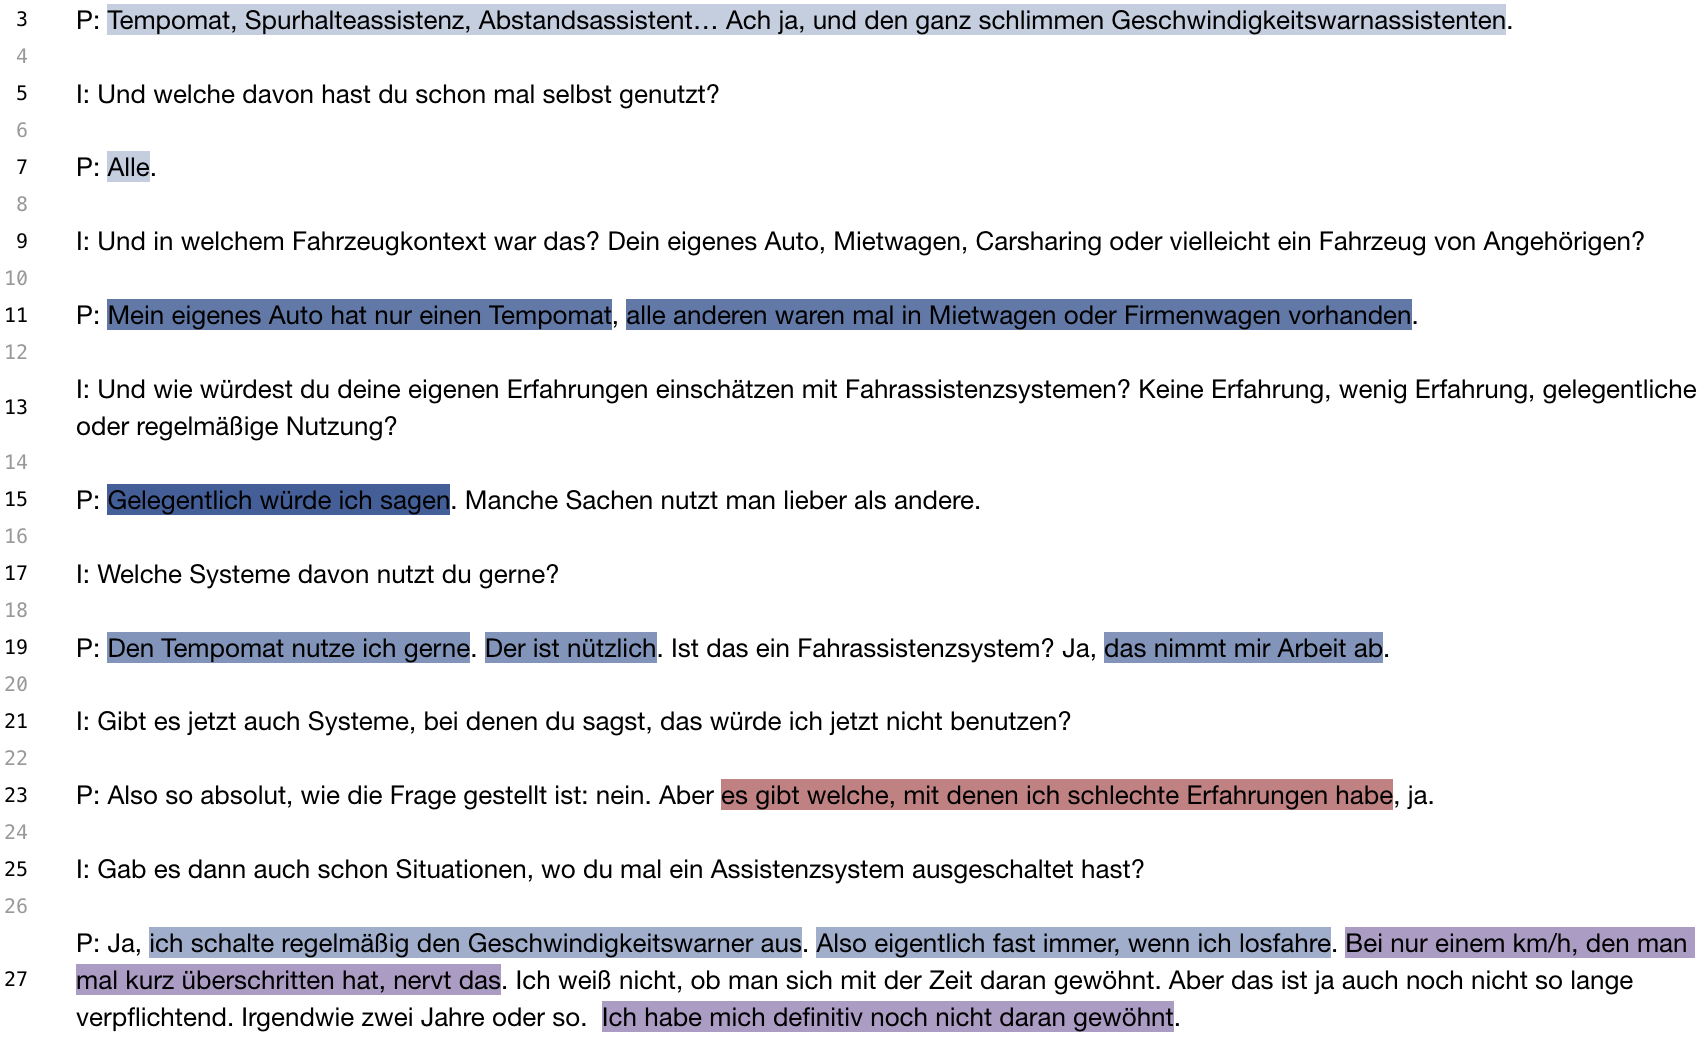
\includegraphics[width=0.7\textwidth]{images/method/OpenQDA_Ausschnitt.png}
    \caption{Ausschnitt aus der Software OpenQDA}
    \label{fig:OpenQDA}
    \medskip
    {\footnotesize Quelle: Eigene Darstellung.}
\end{figure}

Abbildung \ref{fig:Kuckartz} zeigt das Vorgehensmodell der Qualitativen Inhaltsanalyse nach Kuckartz.

\begin{figure}[H]
    \centering
    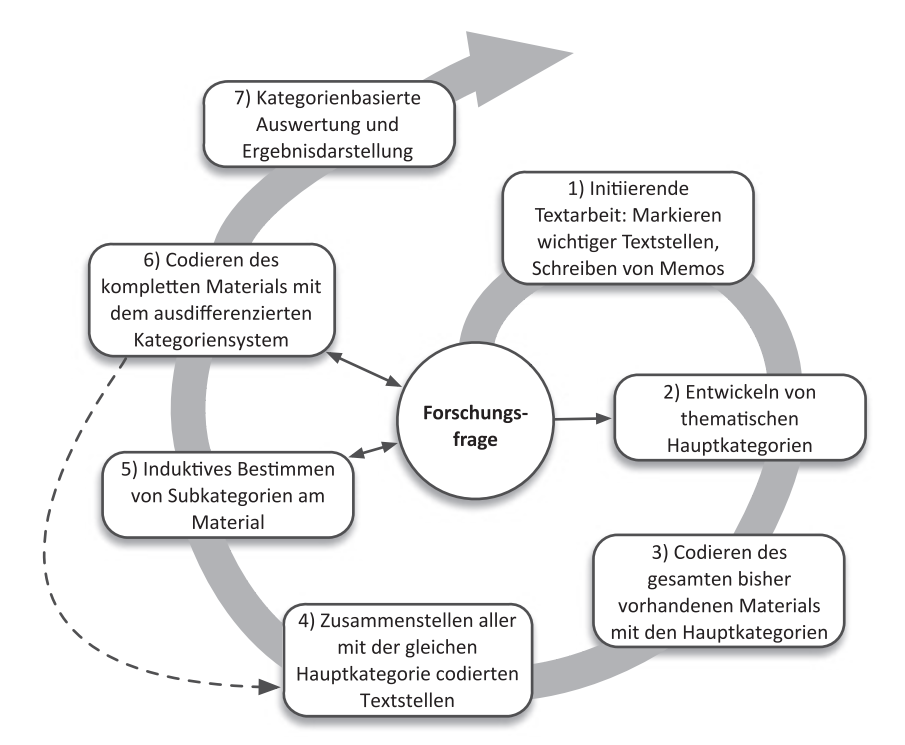
\includegraphics[width=0.7\textwidth]{images/method/Modell_QI.png}
    \caption{Vorgehensmodell der Qualitativen Inhaltsanalyse nach Kuckartz}
    \label{fig:Kuckartz}
    \medskip
    {\footnotesize Quelle: Entnommen aus \cite[S.~111]{kuckartz2014mixed}.}
\end{figure}

\section{Zielsetzung der Lösung}
\label{sec:Methodik_Phase_zwei}

In dieser DSR-Aktivität wurden die verdichteten Befunde aus dem letzten Schritt der qualitativen Inhaltsanalyse den in Kapitel \ref{chapter:theory} herausgearbeiteten Erkenntnissen aus dem Forschungsstand gegenübergestellt. Die Synthese erfolgte entlang gemeinsamer Themenbereiche, beispielsweise Systemverständnis, Systemgrenzen, Fahrer*innenrolle, Informationszeitpunkt und Darstellungsform. Für jedes Synthesethema wurde geprüft, inwieweit Literatur- und Interviewbefunde übereinstimmten, sich ergänzten oder unterschiedliche bzw. widersprüchliche Gestaltungsbedarfe erkennen ließen.

Bei Themen, für die zwar ein grundlegendes Gestaltungsziel erkennbar war, die
konkrete Ausprägung jedoch offen blieb, wurden zusätzlich Spannungsfelder
formuliert. Diese betrafen insbesondere unterschiedliche Präferenzen oder
konkurrierende Gestaltungsziele, beispielsweise den Grad der Führung, den
Umfang der Personalisierung, die Verteilung von Informationen vor und während
der Fahrt sowie die Wahl geeigneter Darstellungsmodalitäten. Solche
Spannungsfelder wurden bewusst nicht durch eine vorab festgelegte
Gestaltungslösung aufgelöst, sondern als offene Gestaltungsfragen in die
nachfolgende partizipative Konzeptentwicklung überführt. 

Auf Grundlage der Synthese wurden anschließend zunächst übergeordnete Designprinzipien in Anlehnung an Gregor et al. \cite{gregor2020anatomy} und Maedche \cite{maedche2019structuring} formuliert. Diese beschreiben in präskriptiver Form, welche grundlegenden Gestaltungsziele das In-Car-Onboarding erfüllen sollte, ohne bereits eine konkrete technische oder gestalterische Umsetzung festzulegen. Abbildung \ref{fig:Schablone_DP} zeigt die Schablone zur Formulierung von Design Prinzipien nach Maedche \cite{maedche2019structuring}.

\begin{figure}[H]
    \centering
    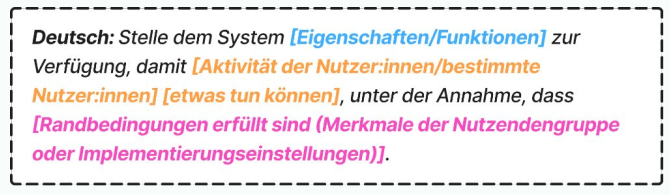
\includegraphics[width=0.8\textwidth]{images/method/Schablone_DP.png}
    \caption{Satzschablonen zur Formulierung von Designprinzipien}
    \label{fig:Schablone_DP}
    \medskip
    {\footnotesize Quelle: Entnommen aus \cite[S.~22]{dogangun2025dsr}.}
\end{figure}

Aus den Designprinzipien wurden in Anlehnung an Iivari \cite{iivari2020critical} und Maedche \cite{maedche2019structuring} anschließend konkrete Design Requirements abgeleitet. Diese spezifizieren, welche Eigenschaften und Funktionen das In-Car-Onboarding aufweisen muss, damit die zuvor formulierten
Designprinzipien umgesetzt werden können. Anforderungen, die sich aufgrund
einer deutlichen Übereinstimmung von Literatur- und Interviewbefunden
eindeutig ableiten ließen, wurden bereits an dieser Stelle festgelegt. Abbildung \ref{fig:Schablone_DR} zeigt ein Template zur Formulierung von Design Requirements nach Maedche \cite{maedche2019structuring}.

\begin{figure}[H]
    \centering
    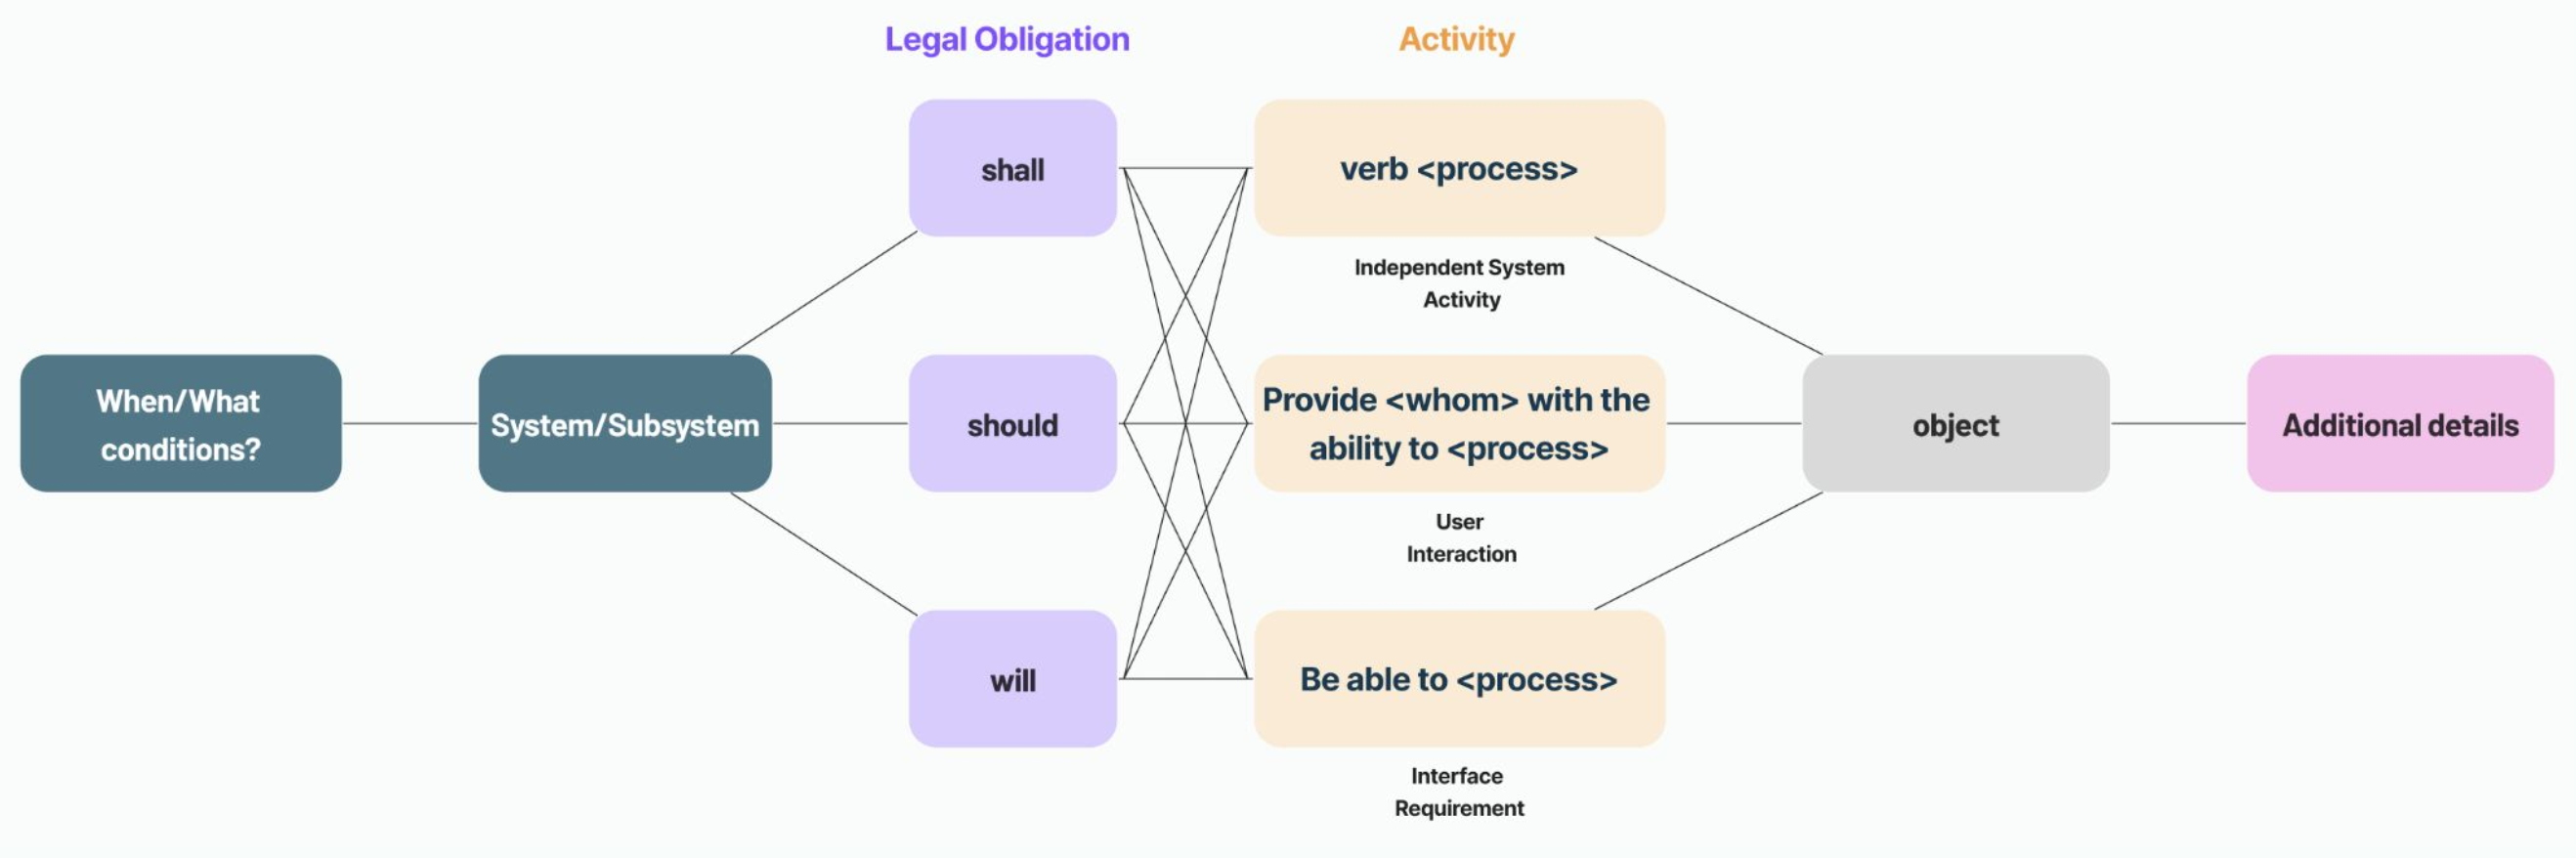
\includegraphics[width=1\textwidth]{images/method/Schablone_DR.png}
    \caption{Template zur Formulierung von Design Requirements}
    \label{fig:Schablone_DR}
    \medskip
    {\footnotesize Quelle: Entnommen aus \cite[S.~26]{dogangun2025dsr}.}
\end{figure}

\section{Design und Entwicklung}
\label{Methodik_Phase_drei}

Auf Grundlage der zuvor abgeleiteten Designprinzipien und Design Requirements
wurden im Rahmen dieser DSR-Aktivität partizipative Workshops durchgeführt. Ziel der Workshops war es, die wissenschaftlich und empirisch begründeten Anforderungen gemeinsam mit potenziellen Nutzer*innen in konkrete Gestaltungsideen für ein In-Car-Onboarding zu überführen. Dabei sollten insbesondere solche Gestaltungsentscheidungen partizipativ konkretisiert werden, deren Ausprägung auf Grundlage von Literatur und Interviews noch nicht eindeutig festgelegt werden konnte.

Die Design Requirements bildeten damit den inhaltlichen Gestaltungsrahmen der
Workshops, während die zuvor identifizierten Spannungsfelder als offene
Gestaltungsfragen in die Workshops eingebracht wurden. Die Teilnehmenden sollten
die zugrunde liegenden Anforderungen nicht grundsätzlich neu bewerten, sondern
innerhalb des vorgegebenen Rahmens mögliche Umsetzungen entwickeln. Ziel war
somit nicht die erneute Anforderungsanalyse, sondern die partizipative
Konkretisierung der Anforderungen in Form potenzieller Design Features.

\subsection{Partizipative Workshops}
\label{subsec:Partizipative_Workshop}

\subsubsection{Stichprobe und Rekrutierung}
Auch für die partizipativen Workshops bildeten die Zielgruppe Personen mit einer innerhalb der Europäischen Union gültigen Fahrerlaubnis. Darüber hinaus wurde auch in diesem Fall eine hinsichtlich des Alters und Geschlechts diverse Zusammensetzung angestrebt. Insgesamt nahmen an den drei Workshops je vier Personen teil, wovon xxx männlich und xxx weiblich waren. Die Altersspanne umfasste 25 bis 64 Jahre. Auch hier erfolgte die Rekrutierung über das persönliche Umfeld und Netzwerke innerhalb der Arbeitsstätte.

\subsubsection{Aufbau und methodische Struktur}
\label{subsubsec:Aufbau_und_methodische_Struktur}

Der Ablauf des Workshops orientierte sich am 4C-Framework nach Courtney
\cite{courtney2020workshopper}. Das Framework strukturiert Workshops anhand der
vier aufeinander bezogenen Schritte 'Collect', 'Choose', 'Create' und 'Commit'. In der Sammelphase werden zunächst unterschiedliche Perspektiven, Herausforderungen und Ideen zusammengetragen. Anschließend werden diese in der Choose-Phase fokussiert und priorisiert. Darauf aufbauend werden in der Create-Phase konkrete Lösungsideen entwickelt, bevor in der Commit-Phase geeignete Ansätze ausgewählt und für die weitere Umsetzung verdichtet werden.

Die vollständigen Workshops umfassten eine Dauer von etwa
120 Minuten und wurde als Präsenzworkshops durchgeführt. Der detaillierte
Leitfaden ist in Anhang \ref{sec:workshopleitfaden} dokumentiert.

\subsubsection{Collect: Erfassung des Problemverständnisses}
\label{subsubsec:Collect}

Zu Beginn der inhaltlichen Arbeit wurden die Informationsbedarfe,
Unsicherheiten und Erwartungen der Teilnehmenden zunächst ohne Vorgabe der
zuvor abgeleiteten Design Requirements erfasst. Hierzu erhielten die
Teilnehmenden ein Szenario, in dem sie sich den erstmaligen Kontakt mit einem
ihnen unbekannten Spurhalteassistenten vorstellen sollten.

In einer zunächst individuellen Arbeitsphase beantworteten die Teilnehmenden
auf Post-its die Frage, welche Informationen oder welches Verständnis sie
für eine sichere und korrekte erste Nutzung der Assistenzfunktion benötigen
würden. Die individuelle Bearbeitung sollte gewährleisten, dass zunächst
eigenständige Perspektiven gesammelt wurden, bevor eine gemeinsame Diskussion
stattfand. Anschließend wurden die Beiträge für alle sichtbar zusammengeführt und inhaltlich unter Zuhilfenahme von Themenkarten, welche sich aus dem Forschungsstand und den abgeleiteten Design Requirements ergaben, gruppiert. Die Themenkarten umfassten den Zweck der Assistenzfunktion, deren Bedienung, Systemstatus, Funktionsweise und Eingriffe, Einsatzbedingungen, Systemgrenzen, die Rolle der fahrzeugführenden Person, Anzeigen und Warnungen sowie das Verhalten bei Systemgrenzen. Die Moderation nahm hierbei keine inhaltliche Bewertung der Beiträge vor.

\subsubsection{Choose: Priorisierung von Inhalten und Informationszeitpunkten}
\label{subsubsec:Choose}

In der anschließenden Choose-Phase wurden die zuvor gesammelten
Informationsbedarfe fokussiert und priorisiert. Zunächst priorisierten die Teilnehmenden die Inhalte individuell mittels Klebepunkten. Darauf aufbauend wurden die Inhalte gemeinsam danach eingeordnet, ob sie mit höchster Priorität vermittelt werden müssen, für den Einstieg hilfreich sind oder erst später beziehungsweise bei Bedarf vertieft werden können.

In einem zweiten Schritt wurde für die priorisierten Inhalte diskutiert, zu
welchem Zeitpunkt eine Vermittlung sinnvoll erscheint. Unterschieden wurde
zwischen Informationen vor der ersten Nutzung, situationsbezogenen
Informationen während der Fahrt sowie Informationen, die später oder bei
Bedarf erneut aufgerufen werden können. Mehrfachzuordnungen waren möglich.
Zusätzlich wurde diskutiert, ob sich der erforderliche Informationsumfang
zwischen den jeweiligen Zeitpunkten unterscheiden sollte.

\subsubsection{Create: Entwicklung konkreter Gestaltungsideen}
\label{subsubsec:Create}

Nach der offenen Sammlung und Priorisierung wurden die zuvor abgeleiteten
Design Requirements in den Workshop eingeführt. Um die Teilnehmenden nicht mit
dem vollständigen wissenschaftlichen Anforderungskatalog zu konfrontieren,
wurden die 14 Design Requirements zu sechs thematisch zusammenhängenden
Gestaltungsrahmen-Karten verdichtet.

Die Karten behandelten die Themen Systemverständnis, Systemgrenzen,
Verantwortung und Vertrauen, Informationszeitpunkt, Darstellung und Warnung
sowie Lernen und Individualisierung. Jede Karte enthielt einen verständlich
formulierten Leitgedanken sowie eine offene Gestaltungsfrage. Die den Karten
zugrunde liegenden Design Requirements blieben dabei erhalten und wurden
dokumentiert, sodass die später entwickelten Gestaltungsideen auf die
wissenschaftlich begründeten Anforderungen zurückgeführt werden konnten.

Gleichzeitig wurden über die offenen Fragen insbesondere diejenigen
Spannungsfelder adressiert, deren konkrete Ausgestaltung in der vorherigen
Synthese nicht eindeutig bestimmt werden konnte. Hierzu zählten beispielsweise
das Verhältnis zwischen verpflichtenden und optionalen Inhalten, der Grad der
Führung, die zeitliche Verteilung der Informationsvermittlung sowie die Wahl
geeigneter Darstellungsmodalitäten.

In der Create-Phase wurden die priorisierten Inhalte, Informationszeitpunkte
und Gestaltungsrahmen in konkrete Lösungsideen überführt. Hierzu arbeiteten die
Teilnehmenden in zwei Kleingruppen mit Paper Prototyping und kleineren Storyboards.

Die Gestaltung erfolgte anhand zweier Nutzungsszenarien. Das erste Szenario
betrachtete den erstmaligen Kontakt mit dem Spurhalteassistenten vor
Fahrtbeginn. Das zweite Szenario adressierte eine Situation während der Fahrt,
in der die Assistenzfunktion aufgrund ungünstiger Rahmenbedingungen, etwa
schlecht erkennbarer oder uneindeutiger Fahrbahnmarkierungen, nicht mehr
zuverlässig unterstützen kann.

Für beide Szenarien sollten die Gruppen bestimmen, welche Informationen
vermittelt werden, zu welchem Zeitpunkt sie erscheinen, wie sie dargestellt
werden und welche Handlung der fahrenden Person vorgesehen ist. Hierfür wurden
Cockpit- und Screen-Vorlagen, Haftnotizen und die zuvor eingeführten
Gestaltungsrahmen-Karten bereitgestellt.

Nach einer ersten Bearbeitungsrunde wechselten die Gruppen das Szenario und
entwickelten eine alternative Lösung für das bisher noch nicht von ihnen bearbeitete Szenario. Die entstandenen Paper Prototypes und Storyboards dienten als Grundlage für
die anschließende Bewertung.

\subsubsection{Commit: Bewertung und Verdichtung}
\label{subsubsec:Commit}

In der abschließenden Commit-Phase wurden die während der Workshops
entwickelten Gestaltungsideen gemeinsam bewertet und verdichtet. Dabei wurde
bewusst nicht zwischen vollständigen Entwürfen abgestimmt. Stattdessen
bewerteten die Teilnehmenden einzelne Gestaltungselemente beziehungsweise
potenzielle Design Features mittels Klebepunkten.

Anschließend wurden besonders geeignete Elemente, kritisch bewertete
Gestaltungsideen, unterschiedliche Präferenzen und weiterhin offene
mehrheitlich unterstützte Gestaltungselemente als auch abweichende Positionen diskutiert.

\subsection{Ableitung der Design Features}
\label{subsec:Ableitung_Design_Features}

Die Ergebnisse der Workshops wurden anschließend in einer Matrix zueinander in Bezug gesetzt und die Gesprächsinhalte zusätzlich systematisch ausgewertet. Im abschließenden Schritt konnten die entwickelten Design Features jeweils auf die zugrunde liegenden Design Requirements sowie auf die Gestaltungselemente der Entwürfe in den Workshops zurückgeführt werden.

Bzgl. der Design Features ist zu beachten, dass von den Proband*innen in den partizipativen Workshops aus zeitlichen Gründen nicht verlangt werden konnte, zwei verschiedene Szenarien so detailliert auszuarbeiten, dass diese sich einerseits mit den Limitationen einer Simulationsumgebung im Einklang befinden und andererseits so umfangreich sind, dass es sich um nahezu perfekte Blaupausen für die konkrete Umsetzung handelt. Stattdessen sollten diese bestmöglich und unter Achtung der Erkenntnisse aus der Literatur sowie vorhandenem Expertenwissen umgesetzt werden. 

\subsection{Gestaltung des Onboardings auf Basis der partizipativen Workshops}
\label{subsec:Gestaltung_Onboarding}

Da die Proband*innen mit dem Onboarding physisch interagieren mussten, um den Design Features, welche den Zeitraum vor Fahrtantritt betreffen, zu entsprechen, wurde ein handelsübliches Tablet (Samsung Galaxy Tab A9 \cite{samsung2023galaxytaba9}) in einem Tabletständer als Substitut für das Display in der Mittelkonsole eines Fahrzeugs genutzt. Die Bedienung zwischen Original und Substitut unterscheidet sich dabei nur marginal, da in beiden Fällen ein Touchscreen zum Einsatz kommt und beide über eine ähnliche Größe verfügen. 

Die zugehörige Android-App, welche ein Fahrzeug-Informationssystem nachbildet, wurde mithilfe des Frameworks Tauri \cite{tauri_dokumentation} entwickelt. Tauri nutzt im Backend die Programmiersprache Rust \cite{klabnik_rust} und für das Frontend ein beliebiges JavaScript-Framework, in diesem Fall React \cite{react_dokumentation}. Diese Entscheidung wurde unter Einbezug von Wartbarkeit und Effizienz getroffen, da unabhängig vom verwendeten Betriebssystem des Entwicklungs- und Zielgerätes nur eine einzige Code-Basis verwendet werden muss. Außerdem bleibt die Dateigröße durch den Rust-Unterbau in einem vertretbaren Rahmen. Das Design der Oberfläche innerhalb der App greift einzelne Gestaltungsideen von Android Auto \cite{google_android_auto} und dem Infotainment-System des Volkswagen-Konzerns \cite{volkswagen_infotainment} auf. Es wurden bewusst große Kacheln verwendet, um die Bedienung für Touchinterfaces zu optimieren. Das Farbschema wurde in Anlehnung an die Farben der Hochschule-Ruhr-West entwickelt. Dabei wurde besonders darauf geachtet, die Farbkontraste ausreichend kräftig zu gestalten und die in Kapitel \ref{subsec:Ergebnisse_Design_Features} vorgestellten Design Requirements bestmöglich in die Gestaltung zu integrieren. Außerdem wurde vergleichbares Infomaterial verschiedener Autohersteller \cite{audi_spurverlassenswarnung,ford_fahrspur_pilot_2021, kia_lane_keeping_assist_2024,mercedes_aktiver_spurhalte_assistent,volvo_pilot_assist_video_guide,volvo_pilot_assist_video_guide,bmw_driver_assistance_settings_2025} zu Spurhalteassistenten gesichtet und ausgewertet.

Das in die Android-App eingebettete Video wurde mithilfe der Videoschnittsoftware Filmora \cite{wondershare_filmora} erstellt. Neben mithilfe der Software Affinity Designer 2 \cite{serif_affinity_designer2} selbst erstellten Grafiken, wurden auch Animationen verwendet, welche aus der Gameengine Unity \cite{unity_engine} exportiert und ebenfalls selbstständig angefertigt wurden. Die Vertonung des Videos erfolgte auf Basis eines eigens entwickelten Skriptes mithilfe einer durch künstliche Intelligenz gestützten Software der Firma Elevenlabs \cite{elevenlabs_text_to_speech}. Diese Entscheidung wurde getroffen, um eine professionelle Vertonung des Videos gewärleisten zu können, da eine deutliche und gleichmäßige Aussprache einzelner Sätze in diesem Kontext von größter Wichtigkeit ist.

Zusätzlich ist auch eine digitale Anleitung in der Android-App enthalten. Diese fasst die wichtigsten Aussagen des Videos noch einmal kompakt zusammen und greift zu diesem Zweck auf Screenshots aus dem Video zurück. Es muss an dieser Stelle betont werden, dass dies ausschließlich als Ergänzung zum Video zu verstehen ist und keinen gleichwertigen Ersatz bietet.

\subsection{Gestaltung eines Fahrzeughandbuches als Vergleichsbedingung}
\label{subsec:Gestaltung_Fahrzeughandbuch}
Um in der späteren Untersuchung die Wirksamkeit des selbst entwickelten Onboardings nachweisen zu können, wurde mithilfe eines selbst angefertigten Fahrzeughandbuches eines realistische Vergleichsbedingung geschaffen. Dieses orientierte sich an frei abrufbaren Anleitungen der Hersteller SEAT \cite{seat_leon_sportstourer_2020}, Opel \cite{opel_astra_2021}, Renault \cite{renault_scenic_2025} und Nissan \cite{nissan_juke_2024} und übernahm teilweise inhaltliche Struktur und einzelne Formulierungen aus diesen, um die Beschaffenheit möglichst realistisch wirken zu lassen.

\subsection{Gestaltung des Fahrsimulators}

Der Fahrsimulator wurde mithilfe der Gameengine Unity \cite{unity_engine} entwickelt. Um ein möglichst realistisches Fahrzeugmodell nutzen zu können, was den Anforderungen (z. B. eigener Bordcomputer) aus den Workshops gerecht werden konnte, wurde ein 3D-Modell \cite{ddiaz_ford_focus_st_2025} eines Ford Focus als Grundlage für das Fahrzeug der Proband*innen genutzt. Das Modell wurde mithilfe der Software Blender \cite{blender_software} umfassend nachbearbeitet und für den Import in Unity angepasst. Da es sich nur um ein Modell ohne jegliche Funktionalität handelte, mussten Fahrphysik, Lichter, Steuerung, Innenraumsteuerung und alle weiteren Funktionen nachträglich ergänzt werden. Besondere Aufmerksamkeit erhielt dabei die Thematik 'Fahrphysik'. Um Forced Feedback mit physikalischen Kräften, welche bspw. im Kontext des Spurhalteassistenten auf das Lenkrad einwirken, bereitstellen zu können, wurde das Unity-DirectInput-Package \cite{imdanoush_unity_directinput} verwendet. Diese öffentlich einsehbare Schnittstelle kann als Alternative zu nur intern verfügbaren Lösungen großer Spielestudios verstanden werden, erreicht aber nicht den gleichen Qualitätsstandard. Abschließend ist es wichtig zu betonen, dass die vom Autor dieser wissenschaftlichen Arbeit geschaffene fiktive Marke 'HRW-Automotive' nicht im Widerspruch zum verwendeten Fahrzeugmodell steht, weil sie sich auf das Informationssystem innerhalb des Fahrzeugs bezieht. 

Auf die Besonderheiten des Spurhalteassistenten innerhalb der Simulation, soll an dieser Stelle kurz eingegangen werden, da die Spurerkennung  eine andere Funktionsweise als in der Realität aufweist. In einem echten Fahrzeug funktioniert ein Spurhalteassistent mithilfe von Kamerasystemen und Bilderkennungsverfahren, welche Abweichungen von der Ideallinie fortlaufend untersuchen \cite{ersoy2025fahrwerkhandbuch}. Zu diesem Zweck ist meist eine kleine Kamera in der Mitte der Windschutzscheibe hinter dem Innenspiegel platziert. Möglich ist auch Infrarot-Sensorik am Unterboden von Fahrzeugen \cite{bubb2015automobilergonomie}. Dieser Ansatz würde innerhalb einer Computersimulation eine vermeidbar hohe Rechenlast erzeugen und führte bei eigenen Tests mit Spezialsoftware \cite{beamng_tech_2025}, welche dieses Prinzip verfolgt, zu unbefriedigenden Ergebnissen. Vor dem Hintergrund des primären Untersuchungsziels dieser Arbeit erscheint es nicht wesentlich, ob die technische Funktionsweise in der Simulation davon abweicht, solange das Ergebnis für die Proband*innen nicht von einem echten Assistenten zu unterscheiden ist. Aus diesem Grund wurde innerhalb der Simulation ein eigener Ansatz verfolgt, der nun kurz erläutert werden soll.

Abbildung \ref{fig:LKA_Demo} zeigt die Visualisierung der Spurerkennung des Assistenten innerhalb der Simulation auf einer in beide Richtungen zweispurigen Autobahn. Durch die perspektivische Verzerrung in der Abbildung scheint es so, dass die Linien nicht vollständig auf den Fahrspurbegrenzungen liegen, obwohl dies tatsächlich zutrifft. Bei den Linien handelt es sich um so genannte Splines, welche mit der Straßengeometrie skalieren. Am oberen Bildrand ist eine leichte Krümmung der Straße zu sehen, welche sich auch im Verlauf der Splines beobachten lässt. Das gesamte Straßennetz ist mithilfe der Splines automatisch karthografiert, sodass das Assistenzsystem keine Bilderkennungsverfahren zur Laufzeit benötigt, da es die Beschaffenheit der Straße kennt. Dieser Ansatz ist innerhalb der Simulation valide, da eine Straße grundsätzlich an jedem Punkt gleich breit ist und die Fahrbahnmarkierungen sich immer an den gleichen Stellen befinden. Mithilfe dieser Methode könnten auch weitere Straßentypen, bspw. Landstraßen erfasst werden, sofern dies im Kontext der wissenschaftlichen Arbeit Relevanz besäße. Die Splines können auch farblich unterschieden werden. Die grünen Splines stellen den Mittelpunkt einer Fahrspur dar. Diese nutzt der Spurhalteassistent, um eine Korrektur der Lenkung vorzunehmen. Die orangene Spline zwischen den beiden grünen Splines 

\begin{figure}[H]
    \centering
    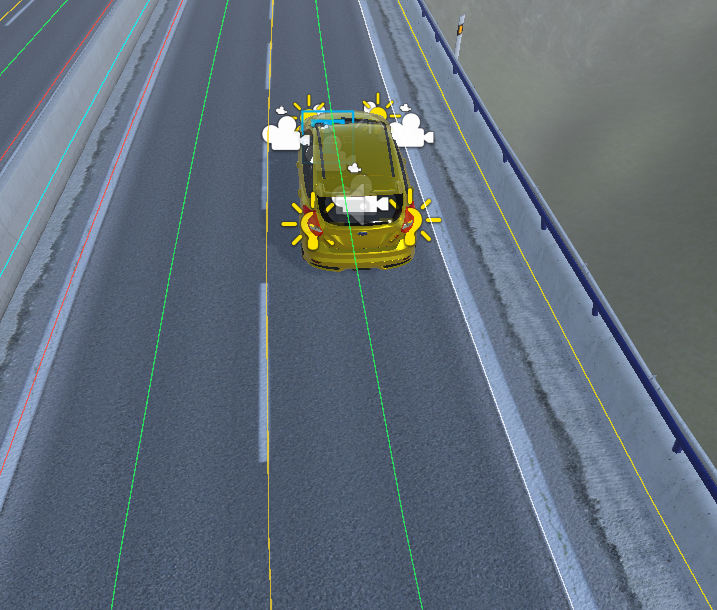
\includegraphics[width=1\textwidth]{images/method/LKA_Demo.png}
    \caption{Illustration der Funktionsweise des Spurhalteassistenten innerhalb des Simulators}
    \label{fig:LKA_Demo}
    \medskip
    {\footnotesize Quelle: Eigene Darstellung}
\end{figure}

Schilder, Symbole und sonstige grafische Elemente wurden ebenfalls mithilfe von Blender \cite{blender_software} oder Affinity Designer 2 \cite{serif_affinity_designer2} angefertigt. Den Design Features entsprechend, ist die Beschaffenheit der Symbole zwischen Onboarding und Simulation bewusst konsistent gehalten. Allerdings muss an dieser Stelle darauf hingewiesen werden, dass die Symbole im Vergleich zu einem echten Fahrzeug etwas größer dargestellt werden. Die Ursache dessen liegt in der starren Perspektive der fahrzeugführenden Person, welche im Vergleich zu einer realen Situation nicht dazu in der Lage ist, die Kopfposition innerhalb der Simulation zu verändern. Es wäre in diesem Fall eine naheliegende Lösung, die Kopfposition innerhalb der Simulation näher am Kombiinstrument zu platzieren. Allerdings würde dies dazu führen, dass die Übersicht über das Verkehrsgeschehen, insbesondere die in diesem Kontext äußerst wichtige Spurführung, darunter leiden würde. Demzufolge wurde ein Kompromiss angestrebt, welcher beiden Anforderungen bestmöglich gerecht werden konnte. 

Für Geräusche wurde auf die freie Soundbibliothek von pixabay \cite{pixabay_soundeffekte} zurückgegriffen, welche anschließend mithilfe der Software Filmora \cite{wondershare_filmora} umfassend nachbearbeitet wurden. Straßen und weitere kontextspezifische Anwendungsfälle betreffend, konnte auf spezielle Packages, bspw. EasyRoads3DPro \cite{andasoft_easyroads3d_pro_2026}, innerhalb von Unity zurückgegriffen werden. Die Wettereffekte wurden mithilfe von passenden Shadern umgesetzt, welche die Illusion von starkem Regen auf den Straßen erzeugen sollten.

\section{Demonstration}
\label{sec:Methodik_Phase_vier}

\section{Evaluation}
\label{sec:Methodik_Phase_fünf}